\documentclass[12pt,slidestop,handout]{beamer}
\usepackage[utf8]{inputenc}
\usepackage{german}
\usepackage{graphicx}
\beamertemplatenavigationsymbolsempty
\usetheme{Boadilla}
\usecolortheme{whale}
\setbeamertemplate{itemize items}[default]
\setbeamertemplate{enumerate items}[default]
\defbeamertemplate*{footline}{my infolines theme} {
\leavevmode
\hbox{
\begin{beamercolorbox}[wd=.333333\paperwidth,ht=2.25ex,dp=1ex,center]{author in head/foot}
\usebeamerfont{author in head/foot}\insertshortauthor
\end{beamercolorbox}
\begin{beamercolorbox}[wd=.333333\paperwidth,ht=2.25ex,dp=1ex,center]{title in head/foot}
\usebeamerfont{title in head/foot}\insertshorttitle
\end{beamercolorbox}
\begin{beamercolorbox}[wd=.309\paperwidth,ht=2.25ex,dp=1ex,center]{date in head/foot}
\usebeamerfont{date in head/foot}\insertshortdate{}\hspace*{2em}
\insertframenumber{} / \inserttotalframenumber\hspace*{2ex}
\end{beamercolorbox}}
\vskip0pt
}
\newcounter{FrameCounter}
\newcommand{\nextframe}[0]{\stepcounter{FrameCounter}}
\newcommand{\framecount}[1]{\frametitle{\arabic{FrameCounter}. {#1}}}
\newcommand{\fitem}{\vfill\item}
\newcommand{\TikZ}{Ti\textit{k}Z}

\title{FSML++}
\author{Carsten Hartenfels \and Benjamin Haßel}
\date{2014-01-09}

\begin{document}
\begin{frame}
	\titlepage
\end{frame}

\begin{frame}
	\frametitle{Contents}
	\pause
	\begin{enumerate}[<+->]
		\fitem Overview
		\fitem Program Structure
		\fitem C++
		\fitem Boost
		\fitem Boost.Spirit.Qi
		\fitem Boost.Format
		\fitem Questions and Answers
	\end{enumerate}\vfill
\end{frame}

\nextframe
\begin{frame}
	\framecount{Overview}\pause
	\begin{itemize}[<+->]
		\fitem Language: C++
		\fitem Parser: Boost.Spirit.Qi
		\fitem Generator: Boost.Format
		\begin{itemize}[<+->]
			\fitem C++ header file
			\fitem \LaTeX/\TikZ\ file
			\fitem Graphviz/Dot file
		\end{itemize}
		\fitem Testing: Google gtest
	\end{itemize}\vfill
\end{frame}

\nextframe
\begin{frame}
	\framecount{Program Structure}\pause
	\vfill
	\begin{center}
		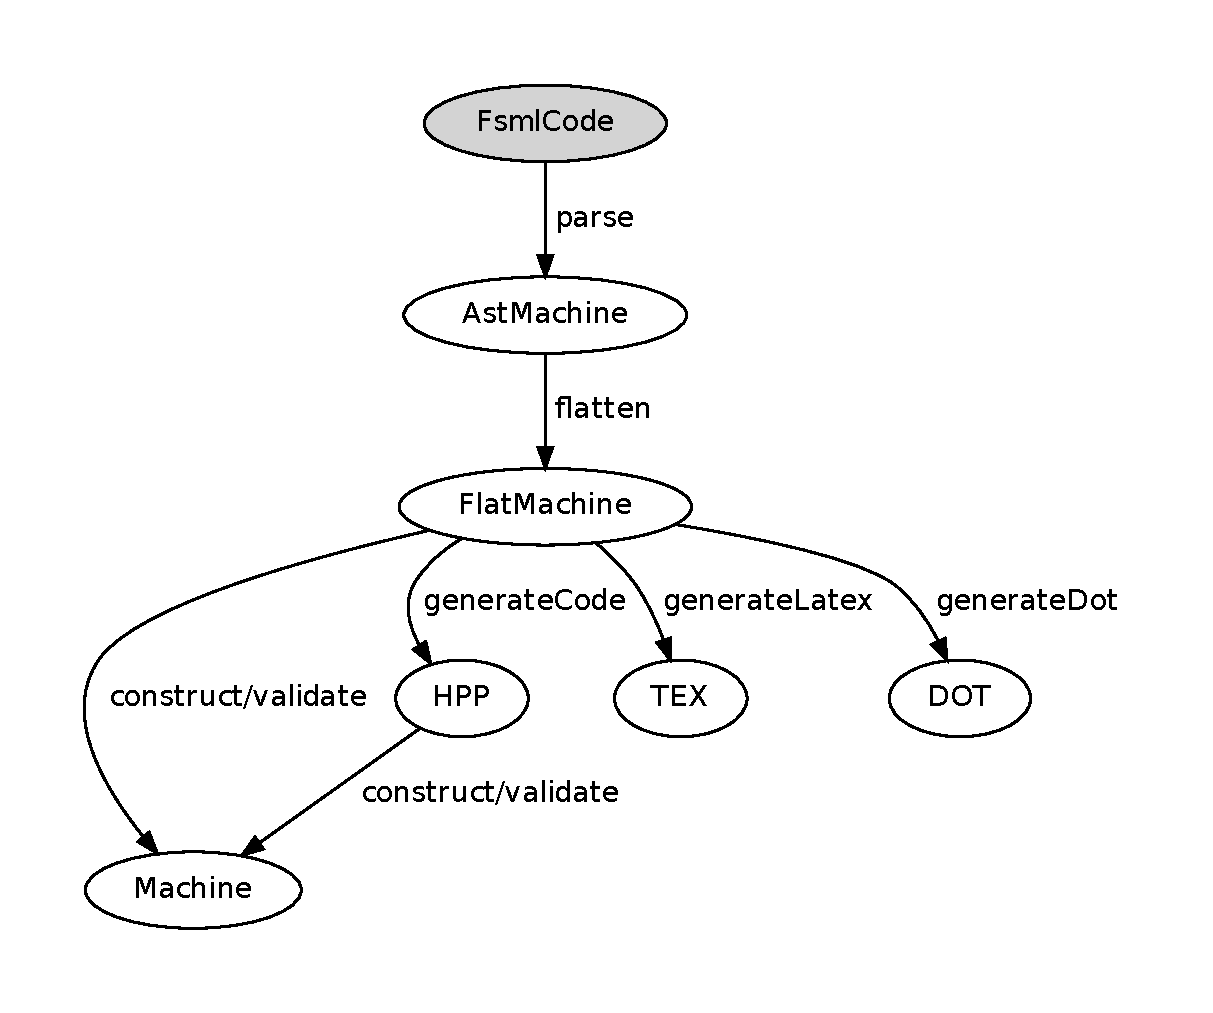
\includegraphics[scale=0.42]{res/Structuredot.pdf}
	\end{center}
	\vfill
\end{frame}

\nextframe
\begin{frame}
	\framecount{C++}\pause
	\begin{itemize}[<+->]
		\fitem Intermediate-Level: No Virtual Machine or Garbage Collection
		\fitem C-Compatible
		\fitem Multi-Paradigm:
		\begin{itemize}[<+->]
			\fitem Procedural
			\fitem Object-Oriented
			\fitem Functional
			\fitem Generic
		\end{itemize}
	\end{itemize}\vfill
\end{frame}

\nextframe
\begin{frame}
	\framecount{Boost}\pause
	\begin{itemize}[<+->]
		\fitem Peer-Reviewed Set of High-Quality Libraries
		\fitem 10 Libraries Adapted Into C++11
		\fitem Used by Adobe, CERN, Google etc.
	\end{itemize}\vfill
\fontsize{6}{1}\selectfont accumulators algorithm any array asio assign atomic bimap bind call\_traits chrono circular\_buffer compatibility compressed\_pair concept config container context conversion coroutine crc date\_time dynamic\_bitset exception enable\_if filesystem flyweight foreach format function function\_types functional functional/factory functional/forward functional/hash functional/overloaded\_function fusion gil geometry graph heap icl identity\_type integer interprocess interval intrusive in\_place\_factory io iostreams iterator lambda lexical\_cast local\_function locale lockfree log math math/complex math/common\_factor math/constants math/floating math/octonion math/special\_functions math/statistical math/quaternion minmax move MPI mpl meta multi\_array multi\_index multiprecision numeric/conversion odeint operators optional parameter Phoenix Predef pointer polygon pool preprocessor program\_options property property proto python random range ratio rational ref regex result\_of scope\_exit serialization signals signals2 smart\_ptr statechart static\_assert spirit string\_algo swap system test thread timer tokenizer TR1 tribool tti tuple type\_erasure type\_traits typeof uBLAS units unordered utility value\_initialized uuid variant wave xpressive\vfill
\end{frame}

\nextframe
\begin{frame}
	\framecount{Boost.Spirit.Qi}\pause
	\begin{itemize}[<+->]
		\fitem Recursive Descent Parser Combinator
		\fitem EBNF-Like Syntax
		\vfill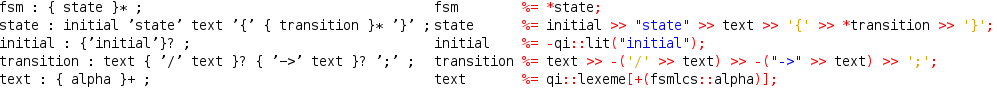
\includegraphics[scale=0.31]{res/ebnfqi.png}
		\fitem DSL Embedded in C++
		\fitem No Code Generation
	\end{itemize}\vfill
\end{frame}

\nextframe
\begin{frame}
	\framecount{Boost.Format}\pause
	\begin{itemize}[<+->]
		\fitem String Formatting
		\fitem Type-Safe
		\fitem Supports User-Defined Types
	\end{itemize}\vfill
	\begin{center}
		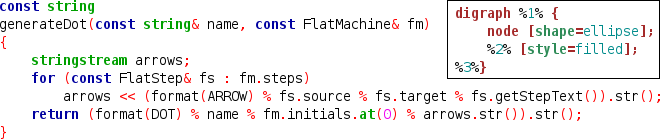
\includegraphics[scale=0.5]{res/format.png}
	\end{center}\vfill
\end{frame}

\nextframe
\begin{frame}
	\framecount{Questions and Answers}
	\begin{center}\vspace{54pt}
		{\Huge Thank You All For Listening}\\\vspace{54.35pt}
		GitHub: \url{https://github.com/hartenfels/FSMLplusplus/}
	\end{center}
\end{frame}
\end{document}
